\documentclass{article}

\usepackage{booktabs}
\usepackage{tabularx}
\usepackage{hyperref}
\usepackage{makecell}   % For multi-line cells
\usepackage{array}     % for custom column formatting
\usepackage{boldline}  % for thicker lines
\usepackage{graphicx}
\usepackage{geometry}
\usepackage{pdflscape}
\usepackage{enumitem}  % For custom numbering of lists
\geometry{a4paper, margin=1in}
\renewcommand{\arraystretch}{1.3} % Adjust row height for better fit

% From: https://tex.stackexchange.com/questions/438876/how-to-cross-reference-text-with-a-custom-label-reference-text
\makeatletter
\newcommand{\labeltext}[3][]{%
    \@bsphack%
    \csname phantomsection\endcsname% in case hyperref is used
    \def\tst{#1}%
    \def\labelmarkup{\emph}% How to markup the label itself
    %\def\refmarkup{\labelmarkup}% How to markup the reference
    \def\refmarkup{}%
    \ifx\tst\empty\def\@currentlabel{\refmarkup{#2}}{\label{#3}}%
    \else\def\@currentlabel{\refmarkup{#1}}{\label{#3}}\fi%
    \@esphack%
    \labelmarkup{#2}% visible printed text.
}
\makeatother

\hypersetup{
    colorlinks=true,       % false: boxed links; true: colored links
    linkcolor=red,          % color of internal links (change box color with linkbordercolor)
    citecolor=green,        % color of links to bibliography
    filecolor=magenta,      % color of file links
    urlcolor=cyan           % color of external links
}

\title{Hazard Analysis\\\progname}

\author{\authname}

\date{October 23, 2024}

%% Comments

\usepackage{color}

\newif\ifcomments\commentstrue %displays comments
%\newif\ifcomments\commentsfalse %so that comments do not display

\ifcomments
\newcommand{\authornote}[3]{\textcolor{#1}{[#3 ---#2]}}
\newcommand{\todo}[1]{\textcolor{red}{[TODO: #1]}}
\else
\newcommand{\authornote}[3]{}
\newcommand{\todo}[1]{}
\fi

\newcommand{\wss}[1]{\authornote{blue}{SS}{#1}} 
\newcommand{\plt}[1]{\authornote{magenta}{TPLT}{#1}} %For explanation of the template
\newcommand{\an}[1]{\authornote{cyan}{Author}{#1}}

%% Common Parts

\newcommand{\progname}{Software Engineering} % PUT YOUR PROGRAM NAME HERE
\newcommand{\authname}{Team \#13, ARC
    \\ Avanish, Ahluwalia
    \\ Russell, Davidson
    \\ Rafey, Malik
    \\ Abdul, Zulfiqar} % AUTHOR NAMES                  

\usepackage{hyperref}
    \hypersetup{colorlinks=true, linkcolor=blue, citecolor=blue, filecolor=blue,
                urlcolor=blue, unicode=false}
    \urlstyle{same}
                                


\begin{document}

\maketitle
\thispagestyle{empty}

~\newpage

\pagenumbering{roman}

\begin{table}[hp]
    \caption{Revision History} \label{rev_history_table}
    \begin{tabularx}{\textwidth}{p{3cm}p{2cm}p{3cm}X}
        \toprule {\textbf{Date}} & {\textbf{Version}} & {\textbf{Author(s)}} & {\textbf{Notes}} \\
        \midrule
        2024-10-23               & 1.0         & All      & Initial Hazard Analysis      \\
        \midrule
        2025-03-24               & 1.1         & Rafey Malik      & Refinements made based on critique      \\
        \midrule
        2025-03-25               & 1.2         & Rafey Malik      & Removed references to the social media aspect of the app      \\
        \bottomrule
    \end{tabularx}
\end{table}

~\newpage

\tableofcontents

~\newpage

\pagenumbering{arabic}

\section{Introduction}

Hazard Analysis is a key step in the engineering process, which is used to identify potential risks and dangers in a system or process. It helps us to ensure the safety and risk management of a system. By systematically analyzing potential risks of the system, we can work to mitigate these potential harms and any consequences that may arise. This document is a key part of the overall safety of the Realm app. It aims to help our stakeholders understand the possible risks of the app and all precautions we have in place to prevent such risks.

\section{Scope and Purpose of Hazard Analysis}

The scope of this Hazard Analysis covers the identification, evaluation, and mitigation of hazards as it relates to the entire development process of the Realm project. A hazard is defined as a property or condition in the system, which when combined with a condition in the environment, has the potential to cause harm or damage. Hazards which are considered in this document include features within the app, and external hazards through the environment. The purpose of hazard analysis is to identify potential hazards in a system early in the design process to mitigate risks and ensure the safety and reliability of the system. \\

Certain losses that could be incurred because of hazards are loss of privacy, including unauthorized tracking of users location and unauthorized sharing of personal data, such as email or password. Another loss is health risks from bright flashes within the app, which can trigger seizures in users that may be suffering from photosensitive epilepsy. Furthermore, human injury may occur from accidents because of users being distracted from AR content.

\section{System Boundaries and Components}

\begin{center}
    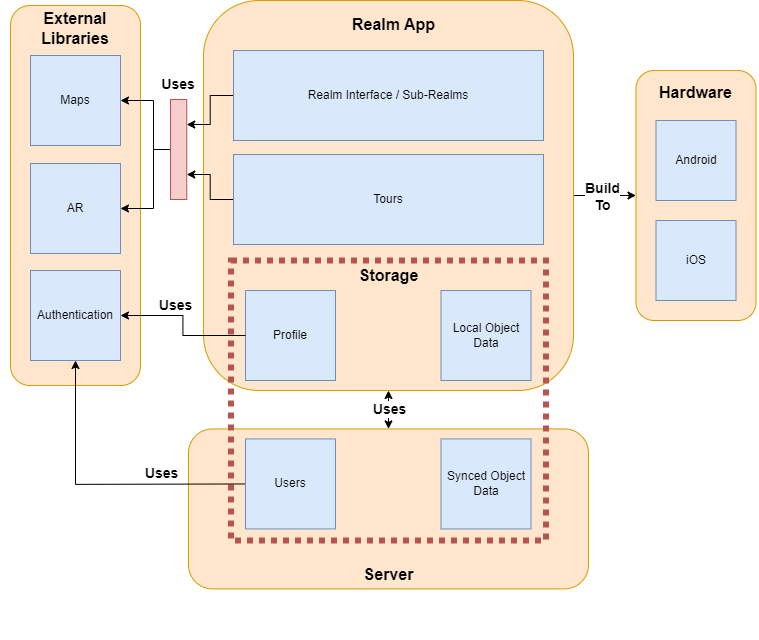
\includegraphics[scale=0.5]{sys_bound_comp.png} \\
    \textbf{Figure 1: System Boundaries and Components}
\end{center}

There are two types of sub-systems that make up the project:
\begin{itemize}
    \item \emph{Internal}: These are sub-systems that are designed and implemented as part of the project.
    \item \emph{External}: These are sub-systems that are created by a third-party.
\end{itemize}

\begin{enumerate}[label=\textbf{\arabic*.}]
    \item \textbf{Realm App}
    \begin{enumerate}
        \item Realm Interface
        \item Tours
    \end{enumerate}
    \textbf{On Failure:} \emph{See \nameref{sub:fmea}}
    \item \textbf{Cloud}
    \begin{enumerate}
        \item Accounts
        \item Synced Object Data
    \end{enumerate}
    \textbf{On Failure:} \emph{See \nameref{sub:fmea}}
    \item \textbf{External Libraries}
    \begin{enumerate}
        \item Maps
        \item AR
        \item Weather
        \item Authentication
    \end{enumerate}
    \textbf{On Failure:} A message will be displayed to inform the user that the app can't connect to a specific service.
    \item \textbf{Hardware}
    \begin{enumerate}
        \item Android Devices
        \item iOS Devices
    \end{enumerate}
    \textbf{On Failure:} The user will get information from the hardware device itself.
\end{enumerate}

\section{Critical Assumptions}

\begin{itemize}
    \item The software system is only used in the intended software environments (unmodified iOS and Android Versions 16.0+ and 12.0+ respectively as per distribution requirement DI-D1)
    \item The software system is only used on devices that meet the minimum hardware requirements (GPS, camera, and all required sensors present)
    \item The user device hardware will not fail for reasons unrelated to the software system
\end{itemize}

\section{Failure Mode and Effect Analysis}
\label{sub:fmea}

\newgeometry{left=0.2in,right=0.2in,top=0.2in,bottom=0.2in}
\begin{landscape}
\begin{table}[hp]
    \caption{FMEA Table} \label{FMEA}
    \centering
    \begin{footnotesize}
    \begin{tabular}{|p{1in}|p{1in}|p{1.5in}|p{1.5in}|p{1.5in}|p{2in}|p{0.4in}|p{0.4in}|}
        \hline
        \multicolumn{1}{|c|}{\textbf{Design Function}} & \multicolumn{1}{c|}{\textbf{Failure Modes}} & \multicolumn{1}{c|}{\textbf{Effects of Failure}} & \multicolumn{1}{c|}{\textbf{Causes of Failure}} & \multicolumn{1}{|c|}{\textbf{Detection}} & \multicolumn{1}{c|}{\textbf{Recommended Action}} & \multicolumn{1}{c|}{\textbf{Req}} & \multicolumn{1}{c|}{\textbf{Ref.}} \\
        \hline
        Object Placement & System fails to store AR object instance in database & User has to redo the object placement workflow, wasting their time & Database failure, Back-end overwhelmed with traffic & Provide useful error messages from back-end to app client & Implement automatic retry mechanism for AR object instance storage in the case of storage failure & \ref{ROR-1}, \ref{ROR-2} & H1-1\\
        \hline
        Object Instance Storage & Database becomes corrupted & Users lose access to their (and other's) AR object instances & Faulty storage devices on server, Bugs in database management software & Automated periodic database testing & Implement a mechanism to restore the database from a backup if necessary, based on automated database testing & \ref{ROR-3}, \ref{ROR-4} & H2-1 \\
        \hline
        Privacy and Data Protection & User data is exposed to unauthorized users & Loss of user trust, potential legal implications, data breaches & Weak encryption, improper access control policies and other security vulnerabilities & Regular security audits, reports of unauthorized access & Implement strong encryption protocols, two-factor authentication, and regular security updates & \ref{SER-1}, \ref{SER-3}, \ref{SER-5} & H3-1 \\
        \hline
        AR Object Rendering &  AR objects fail to render or display incorrectly in the user's environment & Users are unable to see placed objects or experience visual glitches & Device camera issues, insufficient processing power, software bugs, network issues & User-reported issues, monitoring rendering logs & Implement fallback modes for low-performance devices & \ref{ROR-6} & H4-1 \\
        \hline
        Viewing AR objects in the Realm screen & User collides with a real-world object & User is potentially injured, disoriented, and/or damages a real-world object & User is distracted by AR object(s) in the Realm screen and fails to see a real-world hazard right in front of them & Mobile sensors to keep track of user distance from real-world objects & A warning will be displayed through the app when a user is close to an object and is on a collision course & \ref{SAR-1}, \ref{SAR-4} & H5-1 \\
        & & & & & & & \\
        & Location access is disabled & User is unable to accurately view object instances in their surroundings & Permission for location denied by mobile device, Location access disabled by the user, Bugs in software component synchronizing object and device location with each other & Having periodic updates of device location & Prompting user to grant location access or transitioning to an offline view of the Realm screen & \ref{ROR-7}, \ref{SER-6} & H5-2 \\
        & & & & & & & \\
        & User is presented with offensive or obscene content & User has a bad time using the app, or experiences psychological distress & Unmoderated user generated content & User object reports, review process for tours & There should be a system to moderate user generated content based on user reports & (SRS) AI-FR2.1 & H5-3 \\
        & & & & & & & \\
        & Areas are maliciously spammed with objects & Users have a poor viewing experience, people and businesses can be harrassed & Unmoderated user generated content, unrestricted object placement & User object reports & There should be a system to moderate user generated content based on user reports and a system to prevent users from spamming object placements in one location & (SRS) AI-FR2.1, (SRS) OP-FR3 & H5-4 \\
        & & & & & & & \\
        &  User intends to go outside and use the app in bad weather conditions & Increased risk of accidents and injuries due to slippery surfaces, low visibility and other consequences of bad weather conditions & Intense rain/snow/hail, high winds, extreme heat or cold & "Severe weather" warnings using a weather API & Implement warnings for users about adverse weather and encourage them to stay indoors & \ref{SAR-5} & H5-5 \\
        \hline
    \end{tabular}
    \end{footnotesize}
\end{table}
\end{landscape}
\restoregeometry

\newgeometry{left=0.2in,right=0.2in,top=0.2in,bottom=0.2in}
\begin{landscape}
\begin{table}[hp]
    \centering
    \begin{footnotesize}
    \begin{tabular}{|p{1in}|p{1in}|p{1.5in}|p{1.5in}|p{1.5in}|p{2in}|p{0.4in}|p{0.4in}|}
        \hline
        \multicolumn{1}{|c|}{\textbf{Design Function}} & \multicolumn{1}{c|}{\textbf{Failure Modes}} & \multicolumn{1}{c|}{\textbf{Effects of Failure}} & \multicolumn{1}{c|}{\textbf{Causes of Failure}} & \multicolumn{1}{|c|}{\textbf{Detection}} & \multicolumn{1}{c|}{\textbf{Recommended Action}} & \multicolumn{1}{c|}{\textbf{Req}} & \multicolumn{1}{c|}{\textbf{Ref.}} \\
        \hline
        Navigating to AR object cluster & AR objects within selected cluster are deleted by the owner during navigation & User may arrive at destination with no AR objects present, Bugs in navigation software may cause app crashes & All AR objects within the targeted cluster are deleted by respective owners & Keeping track of AR object cluster count & Before starting navigation, check for existence of AR object cluster. Notify user about objects being deleted by owners. Provide option to start navigation back to original starting point & \ref{SAR-6}, \ref{ROR-1} & H6-1 \\
        & & & & & & & \\
        & Location access is disabled & System is unable to present current user location, system is unable to display next instruction & Location access disabled by the user or device system & Having periodic updates of device location & Prompt user to grant location access to continue navigation & \ref{SER-6} & H6-2 \\
        & & & & & & & \\
        & System navigates user to AR object cluster located in a \hyperref[ssub:def]{restricted area}/non-public area & User would be frustrated due to wasted time and effort, user could arrive at a dangerous or harmful area, user could trespass onto private property & System fails to distinguish between restricted and non-restricted areas & Have a record of restricted/private areas, only provide navigation options for unrestricted areas & System denies navigation to the area by notifying the user about the area destination being restricted to the general public & \ref{PVR-1} & H6-3 \\
        \hline
    \end{tabular}
    \end{footnotesize}
\end{table}
\end{landscape}
\restoregeometry

\pagebreak

\section{Safety and Security Requirements}

\subsection{Definitions}
\label{ssub:def}

\begin{enumerate}
    \item \textbf{Encryption standard} \label{encryption standard} - An encryption standard is a set of algorithms used to encode data to ensure that it can be viewed by authorized users only.
    \item \textbf{Restricted Area} \label{restricted area} - A space that should not be accessible to the general public.
\end{enumerate}

\subsection{Safety Requirements}

\begin{enumerate}[label=\textbf{SAR-\arabic*},ref=SAR-\arabic*]
    \item \label{SAR-1} The system should not distract users from their surroundings to the extent that they lose awareness of potential collisions or inadvertently enter restricted areas. \\
    \item \label{SAR-2} The system shall have warnings for bright flashes or loud noises. \\
    \item \label{SAR-3} The system should have the option to disable bright lights and loud noises. \\
    \item \label{SAR-4} The system shall give ample warning to users if they are close to a real-world hazard and on track to collide with it. \\
    \item \label{SAR-5} The system shall display warnings to alert users of going outside during dangerous weather conditions. \\
    \item \label{SAR-6} The system should allow the user to terminate navigation in the Maps component. \\
\end{enumerate}

\subsection{Security Requirements}

\begin{enumerate}[label=\textbf{SER-\arabic*},ref=SER-\arabic*]
    \item \label{SER-1} The system should follow an \hyperref[ssub:def]{encryption standard} for communication between users and with the administrator. \\
    \item \label{SER-2} The system should use a secure method of authenticating user access to system. \\
    \item \label{SER-3} The system shall encrypt all user data stored using an \hyperref[ssub:def]{encryption standard}. \\
    \item \label{SER-4} The system should not reveal the user location to other general users. \\
    \item \label{SER-5} The system shall provide a multi-factor authentication option for user accounts to enhance security. \\
    \item \label{SER-6} The system shall notify the user to grant access to needed device data. \\
\end{enumerate}

\subsection{Robustness Requirements}

\begin{enumerate}[label=\textbf{ROR-\arabic*},ref=ROR-\arabic*]
    \item \label{ROR-1} The system must have an automated mechanism to retry the upload and storage of object instances when an initial attempt fails. \\
    \item \label{ROR-2} All internal APIs of the system must provide useful error messages in the case of system failures. \\
    \item \label{ROR-3} The system must automatically back up databases daily. \\
    \item \label{ROR-4} The system must have a mechanism to restore a database from a backup in the case of unrecoverable failure/corruption. \\
    \item \label{ROR-5} The system shall keep track of object instance count for AR object clusters in the Maps component. \\
    \item \label{ROR-6} The system shall provide fallback modes for rendering AR objects on low-performance devices to ensure accessibility for all users. \\
    \item \label{ROR-7} The system shall have an offline view without location syncing for interactive components. \\
\end{enumerate}

\subsection{Privacy Requirements}

\begin{enumerate}[label=\textbf{PVR-\arabic*},ref=PVR-\arabic*]
    \item \label{PVR-1} The system should be able to identify \hyperref[ssub:def]{restricted areas} and disallow navigation.\\
\end{enumerate}

\section{Roadmap}

\begin{table}[h]
    \centering
    \begin{tabular}{|m{3cm}|m{4cm}|}
        \hline
        \textbf{Requirement} & \textbf{Deadline} \\
        \hline
        \ref{SAR-1} & November 25, 2024 \\
        \hline
        \ref{SAR-2} & November 30, 2024 \\
        \hline
        \ref{SAR-3} & December 5, 2024 \\
        \hline
        \ref{SAR-4} & December 10, 2024 \\
        \hline
        \ref{SAR-5} & December 15, 2024 \\
        \hline
        \ref{SAR-6} & December 20, 2024 \\
        \hline
        \ref{SER-1} & January 1, 2025 \\
        \hline
        \ref{SER-2} & January 6, 2025 \\
        \hline
        \ref{SER-3} & January 11, 2025 \\
        \hline
        \ref{SER-4} & January 16, 2025 \\
        \hline
        \ref{SER-5} & January 21, 2025 \\
        \hline
        \ref{SER-6} & January 26, 2025 \\
        \hline
        \ref{ROR-1} & January 31, 2025 \\
        \hline
        \ref{ROR-2} & February 5, 2025 \\
        \hline
        \ref{ROR-3} & February 10, 2025 \\
        \hline
        \ref{ROR-4} & February 15, 2025 \\
        \hline
        \ref{ROR-5} & February 20, 2025 \\
        \hline
        \ref{ROR-7} & February 28, 2025 \\
        \hline
    \end{tabular}
    \caption{Currently Planned Safety, Security, Robustness, and Privacy Requirements with Deadlines}
    \label{tab:requirements_with_deadlines1}
\end{table}

\begin{table}[h]
    \centering
    \begin{tabular}{|m{3cm}|m{4cm}|}
        \hline
        \textbf{Requirement} & \textbf{Deadline} \\
        \hline
        \ref{ROR-6} & May 30, 2025 \\
        \hline
        \ref{PVR-1} & June 10, 2025 \\
        \hline
    \end{tabular}
    \caption{Future Planned Safety, Security, Robustness, and Privacy Requirements with Deadlines}
    \label{tab:requirements_with_deadlines2}
\end{table}
\newpage{}

\section*{Appendix --- Reflection}

The purpose of reflection questions is to give you a chance to assess your own
learning and that of your group as a whole, and to find ways to improve in the
future. Reflection is an important part of the learning process.  Reflection is
also an essential component of a successful software development process.  

Reflections are most interesting and useful when they're honest, even if the
stories they tell are imperfect. You will be marked based on your depth of
thought and analysis, and not based on the content of the reflections
themselves. Thus, for full marks we encourage you to answer openly and honestly
and to avoid simply writing ``what you think the evaluator wants to hear.''

Please answer the following questions.  Some questions can be answered on the
team level, but where appropriate, each team member should write their own
response:


\begin{enumerate}
    \item What went well while writing this deliverable? \\ \\
    \hspace*{-0.97cm}\textbf{Ans.} Our time management during this deliverable was much better. We decided on much stricter deadlines that were well in advance of the deliverable's deadline, and stuck to them. This allowed us to get most of our main points done 5 days before the deadline. Additionally, we used overleaf and wrote all of our answers in latex, as opposed to writing everything in a Google document and copying it into latex afterwards as we had done for the previous deliverable. This saved us a lot of time and headache by not needing to convert our written text into latex.  \\

    \item What pain points did you experience during this deliverable, and how did you resolve them? \\ \\
    \hspace*{-0.97cm}\textbf{Ans.} When we transferred over to overleaf, we were not able to all work on one combined document and share it with each group member, because this requires access to an overleaf subscription. Instead, we had to create a separate overleaf document for each group member, add our modifications in individually, and then commit them to github via a pull request. This made it much more difficult to see what the final version of the doc would look like before merging everything in github. \\

    \item Which of your listed risks had your team thought of before this
    deliverable, and which did you think of while doing this deliverable? For
    the latter ones (ones you thought of while doing the Hazard Analysis), how did they come about? \\ \\
    \hspace*{-0.97cm}\textbf{Ans.} Some hazards we thought of before this deliverable are moderating obscene content and spamming. Hazards we came up with during this deliverable include tripping and collision, weather hazards, and the user going into restricted areas and private properties. The latter hazards came about while brainstorming, with a focus on more physical, external hazards. This was suggested by our TA, Chris, during our meeting with him. He advised us to include such hazards because our app has some physical component to it, which is that the user goes outside to use the AR features, whereas many software engineering capstone projects do not. \\

    \item Other than the risk of physical harm (some projects may not have any appreciable risks of this form), list at least 2 other types of risk in software products. Why are they important to consider? \\ \\
    \hspace*{-0.97cm}\textbf{Ans.} Security and cultural/psychological hazards. Security hazards are important to consider so that we can protect the data of the user. Our app has access to users' location data, and a data leak can be very harmful to the user, which is why security is very important. Cultural and psychological hazards are important to consider to protect the emotional and social well-being of our users. If this hazard is present, it may discourage the user from using our app, and, depending on the severity of our hazard, may result in legal trouble for the Realm app.\\

\end{enumerate}

\end{document}
